\documentclass{article}

\usepackage[style=ieee]{biblatex}
\usepackage{setspace}
\usepackage{float}
\usepackage{graphicx}
\usepackage{hyperref}
\usepackage{siunitx}
\usepackage{amsmath}

\author{Kian Mehrabani}
\date{April 29, 2021}
\title{Grand Canonical Monte Carlo Simulation of Adsorption Isotherms for Novel Material Discovery}

\bibliography{references}

\begin{document}

\maketitle\newpage
\onehalfspacing

\section{Introduction}
Adsorption is a popular field of research with important applications in catalysis, energy storage systems, and nuclear waste sequestration \cite{h2-storage, sbmof-discovery}.
Key research objectives in this space involve materials discovery to optimize adsorption performance metrics such as adsorption loading at specified conditions and selectivities to target adsorbates.
With the advent of modern computing resources, it is now possible to develop new material structures with the assistance of data from adsorption process simulations and performance indicators form large-scale isotherm data analysis.
In this work, the adsorption isotherm of xenon gas on a novel metal-organic framework (MOF) is simulated using Grand Canonical Monte Carlo (GCMC) simulation methods, then compared with experimental data and a classical adsorption isotherm model. All work is open source and freely available via \texttt{https://github.com/kianmehrabani/adsorption}.

\section{Background}
\subsection{Langmuir Isotherm}
An adsorption process can be modeled as a low-pressure gas in contact with a two-dimensional surface. If the adsorbed gas molecules do not interact on the surface, the canonical partition function for the adsorbed molecules given $N$ distinguishable molecules distributed over $M$ distinguishable adsorption sites is
\begin{equation}
    Q(N, M, T) = \frac{M!}{N!(N-M)!}\left(q_\textit{ad}\right)^N
\end{equation}
where $q_\textit{ad}$ is the partition function for a single adsorbed molecule.
At equilibrium, the chemical potential of the gas will be equivalent to that of the adsorbed molecules, allowing for an analytical expression relating the fractional coverage of adsorbed molecules as a function of temperature, pressure, and the molecular partition functions of both phases,
\begin{equation}
    \theta = \frac{N}{M} = \frac{P}{P + \lambda}
    \label{eq:langmuir}
\end{equation}
where $\lambda = \frac{kT\left(\frac{q}{V}\right)_\textit{gas}}{q_\textit{ad}}$ is known as the Langmuir parameter.
This function is known as the Langmuir isotherm and has a characteristic S shape \cite{iast}.
\begin{figure}[H]
    \centering
    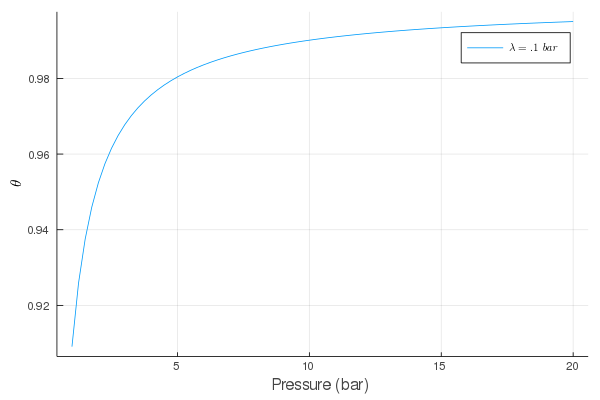
\includegraphics[width=\textwidth]{fig/langmuir.png}
    \caption{Example Langmuir isotherm with langmuir parameter set to .1 bar.}
    \label{fig:langmuir-isotherm}
\end{figure}

\subsection{Grand Canonical Monte Carlo}
Since we are interested in macroscopic properties of real systems, we are free to choose any statistical ensemble since their macroscopic properties are equivalent in the thermodynamic limit.
Because of this, it is most convenient to choose the grand canonical ensemble, which models a system surrounded by a temperature and molecule bath, where molecules may flow in and out of the system while keeping the chemical potential fixed.
This closely models an adsorption process, where a large region of gas in contact with the surface approximates the molecule bath. The partition function for the grand canonical ensemble is
\begin{equation}
    \Xi(\mu, V, T) = \sum_N \exp\left(\frac{N\mu}{k_BT}\right)Q(N, V, T)
    \label{gc-partition}
\end{equation}
where $Q(N, V, T)$ is the canonical partition function.

When sampling states of the grand canonical ensemble, it is more convenient to specify a system pressure, which can be converted to chemical potential.
\begin{equation}
    \mu = \frac{1}{\beta}\ln\left(\beta\Lambda^3f\right)
\end{equation}
where $\beta = \frac{1}{k_BT}$ is the thermodynamic beta, $\Lambda = \sqrt{\frac{h^2}{2\pi mk_BT}}$ is the de Broglie wavelength, and $f = \phi P$ is the fugacity of the gas, a function of pressure \cite{h2-storage}. An equation of state can be used to compute the pure species fugacity at the specified conditions. Alternatively, if the gas pressure is low enough, an ideal gas approximation is sufficient and the fugacity may be replaced with the gas pressure.

Energy fluctuations are simulated by displacement moves similar to canonical Monte Carlo simulations, but molecular fluctuations are allowed in the $\mu$VT ensemble, which are modeled by addition and deletion moves. Addition moves are random insertions on the surface and deletion moves randomly pick an adsorbed molecule and delete it. The acceptance criteria can be derived from a detailed balance, and have the following forms \cite{mol-sim}:
\begin{align}
    \frac{p^\textit{add}_{i\to j}}{p^\textit{add}_{j\to i}} &= \frac{V}{\Lambda^3(N+1)}\exp(-\beta\Delta U + \beta\mu) \\
    \frac{p^\textit{del}_{i\to j}}{p^\textit{del}_{j\to i}} &= \frac{\Lambda^3N}{V}\exp(-\beta\Delta U - \beta\mu)
\end{align}

\section{Methods, Results, and Discussion}
\subsection{Langmuir Isotherm Fitting}
Using \autoref{eq:langmuir}, the langmuir parameter, $\lambda$, was obtained by a linearized curve fit. The linearization of \autoref{eq:langmuir} can be derived by taking the inverse of the equation:
\begin{equation}
    \frac{1}{\theta} = \frac{P+\lambda}{P} = \frac{\lambda}{P} + 1
    \label{eq:linear-langmuir}
\end{equation}
If an adsorption process can be modeled by the Langmuir isotherm, a plot of $\frac{1}{\theta}$ vs. $\frac{1}{P}$ should yield a straight line with a slope of $\lambda$ and an intercept of 1.

The adsorption data reported from the xenon\textendash SBMOF-1 adsorption experiment has units of percent by mass, so the following calculation was performed to convert the adsorption to fractional coverage:
\begin{equation}
    \theta = \frac{N}{M} = \frac{\rho V_\textit{cell}}{\frac{100}{wt\%} - 1}\frac{N_A}{M_\textit{Xe}}
    \label{eq:coverage-conversion}
\end{equation}
\autoref{eq:coverage-conversion} was derived by first converting the mass percentage to weight fraction $\left(\frac{1}{\frac{100}{wt\%} - 1}\right)$. Then the mass of xenon was converted to molecules of xenon $\left(\frac{N_A}{M_\textit{Xe}}\right)$. Finally, the mass of SBMOF-1 was converted to number of unit cells using the crystal density and unit cell volume $\left(\rho V_\textit{cell}\right)$.

The linearized converted experimental data is plotted below.
\begin{figure}[H]
    \centering
    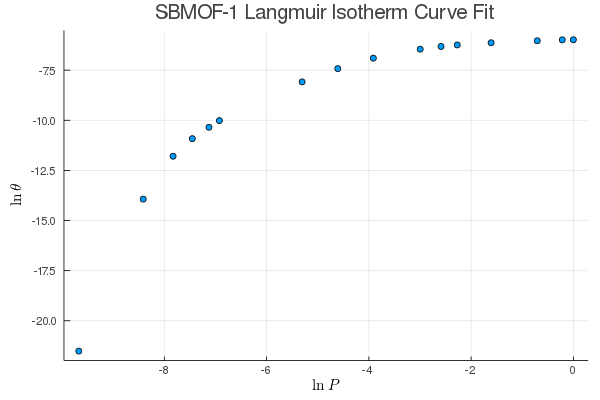
\includegraphics[width=\textwidth]{fig/sbmof1-langmuir.png}
    \caption{Linearized experimental data for the adsorption of xenon gas on SBMOF-1.}
    \label{fig:sbmof1-langmuir}
\end{figure}
Notice that the data in \autoref{fig:sbmof1-langmuir} is not linear, and even neglecting the flat region of the curve, the intercept would not be equal to 1, so this process cannot be modeled by a Langmuir isotherm.
This is due to the disagreement between the physical phenomena and assumptions of Langmuir adsorption.
For instance, there are interactions between adsorbed xenon molecules, which requires a forcefield model to correctly account for.
Also, SBMOF-1 is a porous metal-organic framework, which deviates greatly from an idealized, smooth, two-dimensional surface.

\subsection{Grand Canonical Monte Carlo Simulation}
The \texttt{PorousMaterials.jl} Julia package was used to simulate the adsorption of xenon gas on the novel metal-organic frameworks SBMOF-1 and SBMOF-2 at 298K and a range of pressures from 0 to 1 bar \cite{porous-materials}.
The Peng-Robinson equation of state was used to calculate the xenon fugacity, but since the simulated conditions were at low pressures, this may not have been necessary. A Lennard-Jones potential model was used to model the interactions between adsorbate molecules, using LJ parameters ($\sigma=\SI{3.92}{\angstrom}$, $\frac{\varepsilon}{k_B} = \SI{167}{K}$) from the universal forcefield model \cite{uff}. 5000 each of equilibration and production cycles were executed to find an average adsorption loading. A comparison of the results to experimental data is shown below.
\begin{figure}[H]
    \centering
    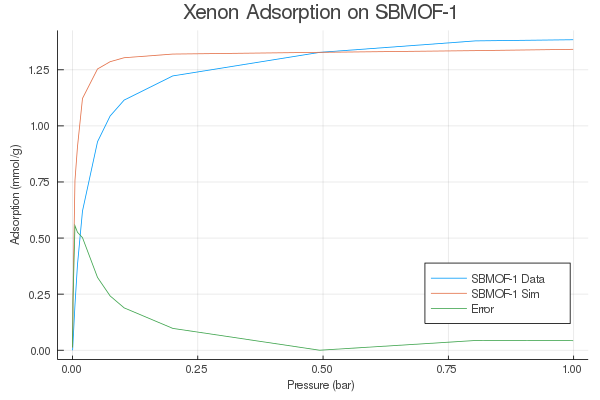
\includegraphics[width=\textwidth]{fig/sbmof1-pengrob-error.png}
    \caption{GCMC simulation adsorption isotherm for xenon gas on SBMOF-1.}
    \label{fig:sbmof1-gcmc}
\end{figure}
\begin{figure}[H]
    \centering
    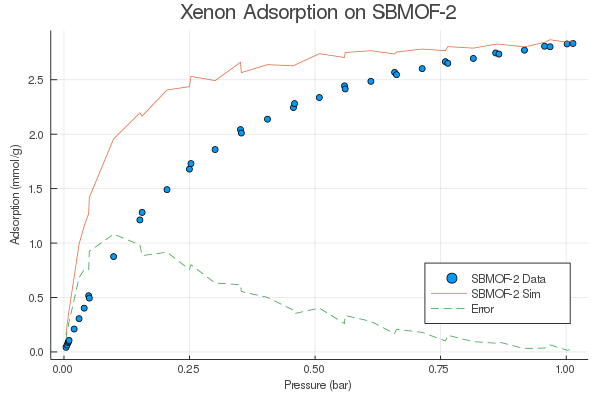
\includegraphics[width=\textwidth]{fig/sbmof2-pengrob-error.png}
    \caption{GCMC simulation adsorption isotherm for xenon gas on SBMOF-2.}
    \label{fig:sbmof2-gcmc}
\end{figure}

The adsorption isotherms in \autoref{fig:sbmof1-gcmc} and \autoref{fig:sbmof2-gcmc} provide a reasonable match to the superimposed experimental isotherms, deviating by around .6\textendash1.1 mmol/g at most.
This accuracy could be improved by adding more production cycles and implementing an energy minimization method as a preliminary step, such as simulated annealing or a gradient descent algorithm.
Nevertheless, these simulations would still prove useful in the design of future novel adsorption materials.

\section{Conclusion}
Simulations of adsorption isotherms of xenon gas on novel metal-organic frameworks were performed using Grand Canonical Monte Carlo (GCMC) methods.
The results compared reasonably well with experimental data, with longer simulation times and energy minimization methods suggested for increased accuracy.
The lack of applicability of a simplified analytical isotherm model, the Langmuir isotherm, was also discussed, with linearized curve fitting methods providing unacceptable fits to experimental data due to nonidealities of complex framework structures and adsorbate lateral interactions.
These simulation methods, combined with the growing digitization of isotherm data, such as the NIST ISODB API, may provide the groundwork for data-driven adsorption materials discovery, perhaps via deep learning techniques. \cite{mining, materials-ml}.

\printbibliography

\end{document}
